\documentclass[tikz,border=4pt]{standalone}
\usepackage[T1]{fontenc}
\usepackage[utf8]{inputenc}
\usepackage{mathptmx}
\usepackage{tikz}
\usetikzlibrary{arrows.meta,positioning,fit,backgrounds}

\definecolor{headcol}{HTML}{E2EAF4}

\begin{document}
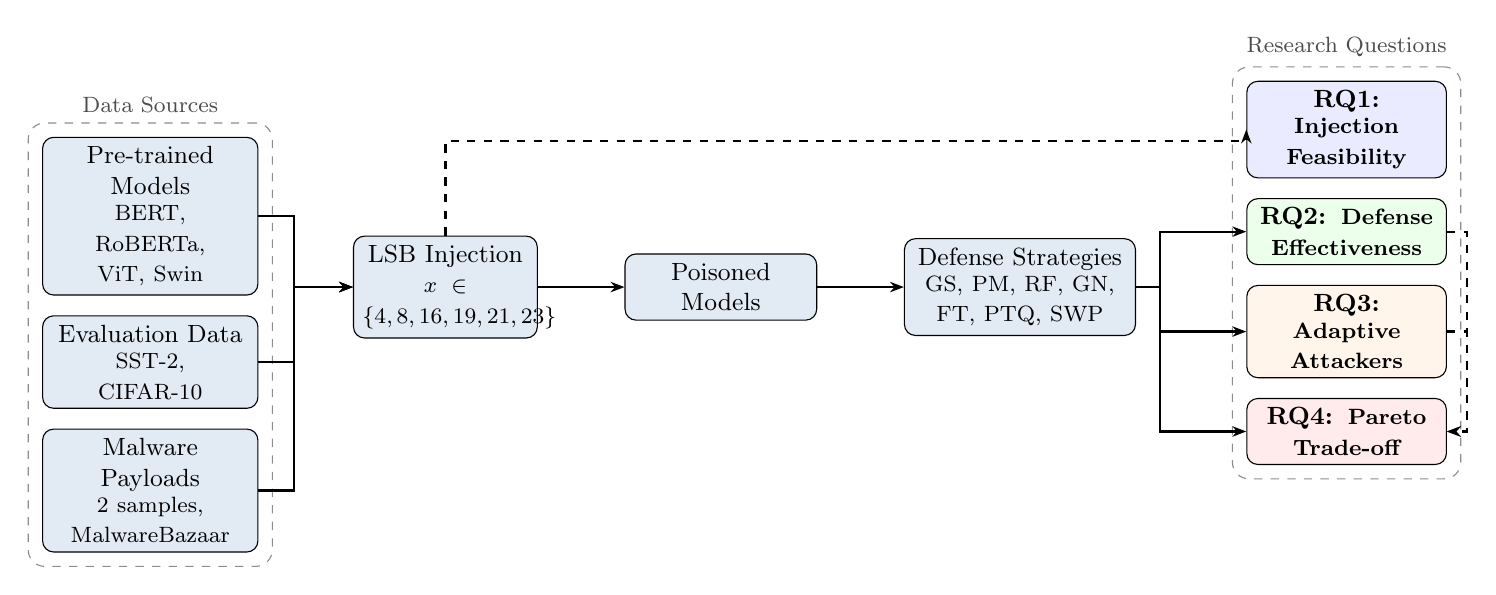
\begin{tikzpicture}[
  font=\small,
  node distance=0.35cm and 0.5cm,
  box/.style={draw,rounded corners=4pt,minimum height=0.65cm,
              text width=2.1cm,align=center,fill=headcol,font=\small},
  rqbox/.style={draw,rounded corners=4pt,minimum height=0.65cm,
                text width=2.3cm,align=center,font=\small\bfseries},
  arr/.style={-{Stealth[length=5pt]},thick},
  darr/.style={-{Stealth[length=5pt]},thick,dashed},
]
\node[box, text width=2.5cm, yshift=2.65cm] (models)
  {Pre-trained Models\\{\footnotesize BERT,\\RoBERTa, ViT, Swin}};
\node[box, text width=2.5cm, below=0.25cm of models] (data)
  {Evaluation Data\\{\footnotesize SST-2,\\CIFAR-10}};
\node[box, text width=2.5cm, below=0.25cm of data] (mal)
  {Malware Payloads\\{\footnotesize 2 samples,\\MalwareBazaar}};

\node[box,text width=2.1cm,right=1.2cm of models,yshift=-0.9cm] (lsb)
  {LSB Injection\\{\footnotesize $x\in\{4,8,16,19,21,23\}$}};

\node[box,text width=2.2cm,right=1.1cm of lsb] (poison)
  {Poisoned\\Models};

\node[box,text width=2.7cm,right=1.1cm of poison] (defenses)
  {Defense Strategies\\{\footnotesize GS, PM, RF, GN,\\FT, PTQ, SWP}};

\node[rqbox,fill=blue!8, right=1.4cm of defenses, yshift=2.0cm] (rq1)
  {RQ1: {\footnotesize Injection\\Feasibility}};
\node[rqbox,fill=green!8, below=0.25cm of rq1] (rq2)
  {RQ2: {\footnotesize Defense\\Effectiveness}};
\node[rqbox,fill=orange!8, below=0.25cm of rq2] (rq3)
  {RQ3: {\footnotesize Adaptive\\Attackers}};
\node[rqbox,fill=red!8, below=0.25cm of rq3] (rq4)
  {RQ4: {\footnotesize Pareto\\Trade-off}};

\draw[arr] (models.east) -- ++(0.45,0) |- (lsb.west);
\draw[arr] (data.east)   -- ++(0.45,0) |- (lsb.west);
\draw[arr] (mal.east)    -- ++(0.45,0) |- (lsb.west);
\draw[arr] (lsb) -- (poison);
\draw[arr] (poison) -- (defenses);

\draw[darr] (lsb.north) -- ++(0,1.2) -| (rq1.west);
\draw[arr] (defenses.east) -- ++(0.3,0) |- (rq2.west);
\draw[arr] (defenses.east) -- ++(0.3,0) |- (rq3.west);
\draw[arr] (defenses.east) -- ++(0.3,0) |- (rq4.west);
\draw[darr] (rq2.east) -- ++(0.25,0) |- (rq4.east);
\draw[darr] (rq3.east) -- ++(0.25,0) |- (rq4.east);

\begin{scope}[on background layer]
  \node[draw=gray!90,dashed,rounded corners=6pt,
        fit=(models)(data)(mal),
        inner xsep=5pt,inner ysep=5pt,
        label={[font=\footnotesize,black!70]above:Data Sources}] {};
  \node[draw=gray!90,dashed,rounded corners=6pt,
        fit=(rq1)(rq2)(rq3)(rq4),
        inner xsep=5pt,inner ysep=5pt,
        label={[font=\footnotesize,black!70]above:Research Questions}] {};
\end{scope}
\end{tikzpicture}
\end{document}
